\section{Enrichment Overview}
% Paper 2
In this context the term enrichment describes the extension of the (semantic)
schema of a knowledge base. The process of knowledge base enrichment increases the
semantic richness and the expressiveness of an ontology. 
The goal of the enrichment progress is to find axioms, which can be added to an
existing ontology. A special case is to find definition of classes and
subclasses. This process is closely related to the Inductive Logic Programming
(ILP) as it is described later in this report.
Ontology enrichment methods usually depend on machine learning or on applying
heuristics to find additional axioms in the knowledge graph.\cite{paper2}

As stated before, knowledge base enrichment usually work on existing data to
improve the semantic schema. It supports the so called \emph{grass-root}
approach for creating ontologies. Here the whole ontology structure is not
created upfront, but evolves over time and with every part of data that is added to the
knowledge base.\cite{paper2}

% % Liste approaches
% - description logic: least common subsumer
% - top-down, refinement operator for ALER 
% - combine in YINYANG tool 
% 
% % Paper2: p60
% - knowledge base completetion (well-defined sense) classes <-> subclasses 
% 
% - CELOE (heuristics and adaptation), described later

\begin{figure*}
\centering
\label{venn}
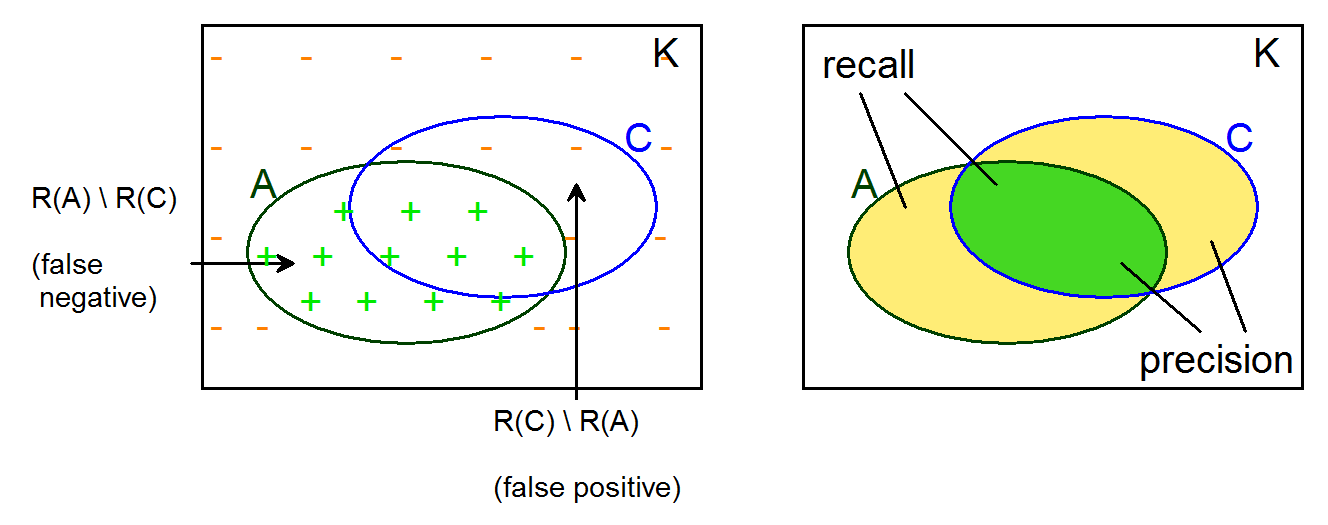
\epsfig{file=img/venn.png, width = 14 cm}
\caption{This figure visualises the class $A$ and the expression to test $C$ as
a Venn diagram. It also shows the the terms \emph{recall} and \emph{precision}.}
\end{figure*}



%=====================================================================================
%=====================================================================================
%=====================================================================================
\newpage
\section{Class Learning}
% Paper 1
\subsection{Motivation}
The class learning approach is one method of enrichment of knowledge bases. It
aims at finding new definition of classes to extend the semantic schema. For the
motivation of the method consider the following example.

\begin{example}
For this example consider a knowledge base containing a class \emph{President of
the United States} with instance data like Abraham Lincoln, John F. Kennedy,
Bill Clinton and Barack Obama. A class Learning algorithm may suggest that the
President class is equivalent to the following two class expressions:
\\\hspace*{12pt}\texttt{1) Person and born in the USA}\\
\hspace*{12pt}\texttt{2) American citizen and born in the USA}\footnote{The
class 'American citizen' is here a subclass of 'Person', which makes the second
statement more specific.}
\end{example}

These suggestions would then be presented to a knowledge engineer who than can
decide if they are plausible and therefore should be added to the knowledge
graph or should be discarded.
Should the engineer for instance choose the second statement, he could check if
there are instances of the class \emph{President}, where the individual is not
of type American citizen. This could indicate an error or missing information in the
knowledge graph which could then be fixed in this semi-automated approach by the
knowledge engineer.


\subsection{Learning Problem}
The problem of learning class definitions for given data depend on the so called
inductive reasoning as opposed to inference or deductive reasoning. \cite{paper1}
Inductive Reasoning is also a key concept in Inductive Logic Programming.

\newdef{definition}{Definition}
\begin{definition}
We are searching for a formal description of the class $A$, which has existing
instances in the examined ontology. A possible class expression $C$ then
contains axioms of the form $A \subseteq C$ or $A \equiv C$.
\end{definition}

This means that the learned expression $C$ is a description of the individuals
of $A$. In our president example, the individuals are the presidents John F.
Kennedy, Barack Obama etc. whereas $C$ can be one of the suggested expression.
In many cases there will be no exact solution for $C$, but rather an
approximation. This can be the case, if the knowledge base contains false class
assignments or missing information. In our example the birthplace of Thomas
Jefferson might be missing in the ontology. However, if most of the other
presidents have the correct birthplace the learning algorithm may still suggest
the expressions. Again, missing information may be completed by the knowledge
engineer.

In a complex knowledge base a class learning algorithm may find many new class
definition and often different expression for the same class. Based on Occam's
razor \cite{occam-razor} simple solutions are preferred over complex ones,
because they are more readable an thus easier for the knowledge engineer to
evaluate. Simplicity is measured in an straight forward way: the length of an
expression, which consists of role, concept and quantifiers.
The algorithm is biased towards shorter expressions. \cite{paper1}

\subsection{Algorithm}
One algorithm for solving the learning problem is called CELOE (Class
Expression Learning for Ontology Engineering). It is described in \cite{paper1}.
An brief overview of CELOE is given in Figure 2.
\begin{figure}
\label{celoe}
\centering
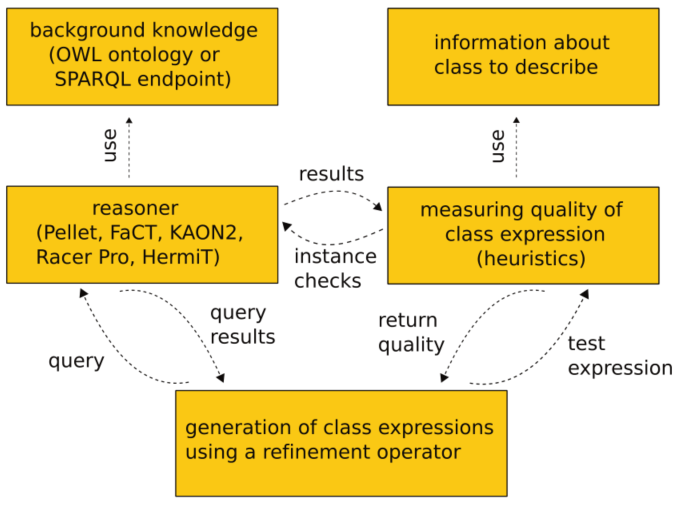
\epsfig{file=img/celoe.png, width = 8 cm}
\caption{CELOE\cite{paper1}}
\end{figure}
The algorithm follows the ``generate and test'' approach which is the common
concept in ILP. \cite{Foundation_ILP} 
In the learning process many class expression are created and tested against the
background knowledge. Each of these class expressions is evaluated using
different heuristics, which are described in detail in a separate section.

To find appropriate class expression to describe existing classes CELOE uses a so
called \emph{refinement operator}. The idea of these operator is based on the
work in \cite{refinement1},\cite{refinement2} and \cite{refinement3}. Refinement
operators are used to search in the space of expressions. It can be seen as a
top-down algorithm as it is illustrated in Figure 3.
As an example consider the following path ($\leadsto$ indicates a refinement
step):\vspace{6pt}\\
$T \leadsto Person \leadsto Person \sqcap takesPartIn.T \leadsto Person \sqcap
takesPartIn.Meeting$

\begin{figure}
\label{tree}
\centering
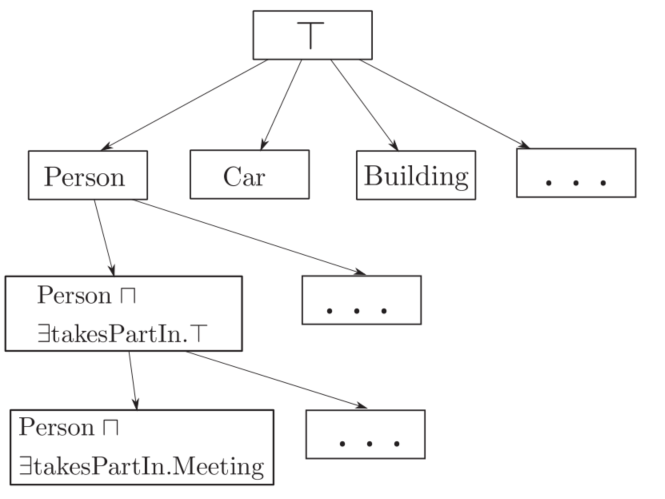
\epsfig{file=img/tree.png, width = 8 cm}
\caption{Tree\cite{paper1}}
\end{figure}


%=====================================================================================
%=====================================================================================
%=====================================================================================
\newpage
\section{Enrichment with OWL Axioms}
% Paper 2
OWL offers many different types of axioms for a method to enrich the knowledge
base. 
\begin{figure}
\label{3-Phase}
\centering
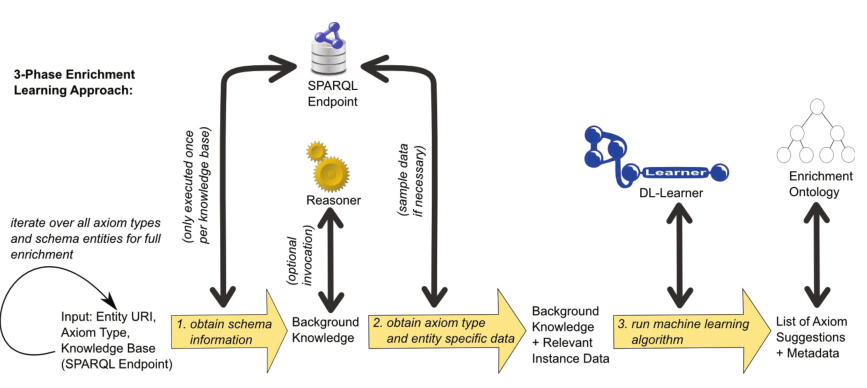
\epsfig{file=img/3-phase-enrichment.png, width = 8 cm}
\caption{3-Phase Enrichment Workflow\cite{paper2}}
\end{figure}
Figure \ref{3-Phase} shows the 3 steps in the enrichment workflow as described
in \cite{paper2}:
\begin{enumerate}
  \item The first phase is about obtaining general information about the
  knowledge base, in particular axioms, which define the class hierarchy are
  obtained. The schema queried via SPARQL, but is loaded only once.
  \item In the second phase data is again obtained via SPARQL. These background
  checks allows the method to learn and test new axioms. Examples for axiom
  types are explained in the following text.
  \item The score of axiom candidates is computed and the result is returned.
\end{enumerate}

The algorithm for suggestion of new axioms is based on checking and counting RDF
triples. In the following example we want to learn if the class $A$ is an
appropriate domain of a predicate $p$. For that we count the triples that match
this statement to obtain a score. 

\begin{example}
Lets look at the predicate \texttt{onto:attendsMeeting} and check if we can find
a suitable candidate for a domain. Note that \texttt{onto:Manager} is a subclass
of \texttt{onto:Employee}.
\end{example}
\begin{lstlisting}[morekeywords={onto, rdf, rdfs}, caption=Triples written in
turtle syntax] @PREFIX onto: <http://ontology-to-enrich.com/>.
onto:Software_Engineer		
		onto:attendsMeeting 	onto:TeamMeeting;
		rdf:type				onto:Employee.
onto:Software_Architekt		
		onto:attendsMeeting 	onto:TeamMeeting;
		rdf:type				onto:Employee.
onto:Project_Manager		
		onto:attendsMeeting 	onto:ManagerMeeting;
		rdf:type				onto:Manager.
		
onto:Manager   rdfs:subClassOf	onto:Employee.
\end{lstlisting}
Looking at this example we would obtain a score of 33.3 \% (1 out of 3) for the
class \texttt{onto:Manager} and 100 \% (3 out of 3) for the class
\texttt{onto:Employee}.\\
Obviously this extreme simple and straightforward method of calculating the score
for the domain of a predicate $p$ has some limitation.
Mainly the method doesn't discriminate between a score calculated by having 100
out of 100 correct observations or only 3 out of 3. Different methods, for
example the Wald method \cite{wald-methods}, overcome that problem. 
More involved heuristics are shown in the next section. 

\subsection{Obtaining Axioms via SPARQL queries}
This section explains how SPARQL queries are used to extract information in step
2 of the enrichment workflow.

%===============================================================================
%===========================     TABLE     =====================================
% ==============================================================================
\begin{table*}[ht]
\centering
\label{table-heuristic}
\caption{Heuristics}
\begin{tabular}{p{3.5 cm} p{3.5 cm} p{2 cm} p{2 cm} p{2 cm} p{2 cm}} \hline
\textbf{Illustration} & \textbf{accuracy \& recall} & \textbf{pred. acc.} &
\textbf{F-Measure} & \textbf{A-Measure} & \textbf{Jaccard}\\
\hline\hline

\raisebox{-.5\height}{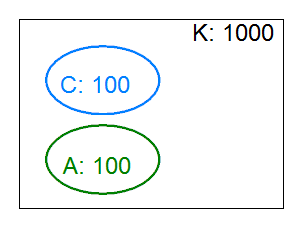
\includegraphics[scale=0.3] {img/table-img1.png}}
& 
\begin{tabular}{l l}accuracy& 0\%\\\\ recall & 0\%\end{tabular}
& 80 \% & 0 \% & 0 \% & 0 \% \\ \hline 

\raisebox{-.5\height}{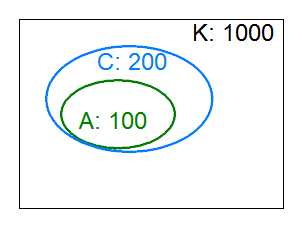
\includegraphics[scale=0.3] {img/table-img2.png}}
&
\begin{tabular}{l l}accuracy& 50\%\\\\ recall & 100\%\end{tabular}
& 90 \% & 66.7 \% & 75 \% & 50 \% \\ \hline 

\raisebox{-.5\height}{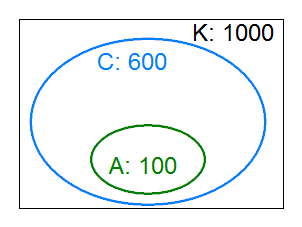
\includegraphics[scale=0.3] {img/table-img3.png}}
& 
\begin{tabular}{l l}accuracy& 16.7\%\\\\ recall & 100\%\end{tabular}
& 50 \% & 28.6 \% & 58.3 \% & 16.7 \% \\ \hline 


\raisebox{-.5\height}{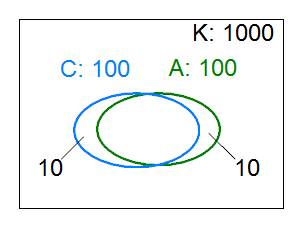
\includegraphics[scale=0.3] {img/table-img4.png}}
& 
\begin{tabular}{l l}accuracy& 90\%\\\\ recall & 90\%\end{tabular}
& 98 \% & 90 \% & 90 \% & 81.8 \% \\ \hline 

\raisebox{-.5\height}{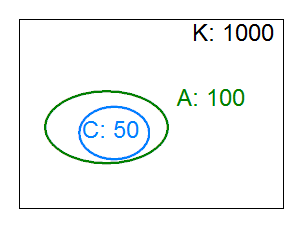
\includegraphics[scale=0.3] {img/table-img5.png}}
& 
\begin{tabular}{l l}accuracy& 50\%\\\\ recall & 100\%\end{tabular}
& 95 \% & 66.7 \% & 75 \% & 50 \% \\ \hline 

\end{tabular}
\end{table*}

\subsubsection*{Subclass and Disjointness of classes}
This query evaluates all individuals (\texttt{?ind}) and checks if they are
instance of the user defined class definition in \texttt{\$class}. In this query
higher count indicates a better candidate for a superclass. 
Lower value indicates a disjointness.
 
\begin{lstlisting} 
SELECT ?type (COUNT(?ind ) AS ?count ) WHERE {
	?ind a <$class >.
	?ind a ?type .
} GROUP BY ?type
\end{lstlisting}

\subsubsection*{Subsumption and Disjointness of properties}
A somewhat similar query can be used to learn subsumption and disjointness of
predicates.

\begin{lstlisting} 
SELECT ?p (COUNT(? s ) AS ?count ) WHERE {
	?s ?p ?o .
	?s <$property> ?o .
} GROUP BY ?p
\end{lstlisting}

\subsubsection*{Domain and Range of properties}
A query for the domain of a property counts the occurrences subjects of type
\texttt{?type} having the property \texttt{\$property}.

\begin{lstlisting} 
SELECT ?type COUNT(DISTINCT ?ind ) WHERE {
	?ind <$property> ?o .
	?ind a ?type .
} GROUP BY ?type
\end{lstlisting}

The query for the range of \texttt{\$property} is analog. It can be also
distinguished between object and data properties. Here only the queries for
object properties are listed.
\begin{lstlisting} 
SELECT ?type (COUNT(DISTINCT ?ind ) AS ?cnt ) WHERE {
	?s <$property> ? ind .
	?ind a ?type .
} GROUP BY ?type
\end{lstlisting}


\subsubsection*{Inverse of Properties}
To check if a property is inverse we check the \texttt{\$property} with subject
and object and in swapped position. As always we count how often the expression
holds.
\begin{lstlisting} 
SELECT ?p (COUNT(*) AS ?count ) WHERE {
	?s <$property> ?o .
	?o ?p ?s .
} GROUP BY ?p
\end{lstlisting}


%=====================================================================================
%=====================================================================================
%=====================================================================================
\section{Heuristics}
% Paper 1


\subsection{Finding the right heuristic}
A heuristic measures how well a given class expression fits the learning
problem. \cite{paper1}
To test an algorithm we must have positive and negative examples. As we want to
describe class $A$ with $C$ we can consider every instance of $A$ as a positive
and everything else as negative examples.
The predictive accuracy can be described as:\vspace{6pt}\\
\centerline{
$
predacc(C) = 1 - \frac{|R(A) \setminus R(C)| + |R(C) \setminus R(A)|}{n} \quad n
= |Ind(K)| $
}\vspace{6pt}
Here, Ind(K) stands for the set of individuals in the knowledge base. $R(A)
\setminus R(C)$ are the false negatives whereas $R(C) \setminus R(A)$ are the
false positives. \\
As you can see in Figure \ref{venn} for the term \emph{precision} we
consider the intersection of $A$ and $C$ ($R(A) \cap R(C)$) and the false
positive. In other words, how many individuals are rightful considered with our
class expression $C$.\\
For the other term \emph{recall} we consider again the intersection of $A$ and
$C$ and the false negative. This score tells us how many individuals of $A$ we
can describe with our class expression $C$.

Table \ref{table-heuristic} compares the score of four different heuristics.
They are:
\begin{itemize}
  \item{\textbf{pred. acc.}} The formula for the predictive accuracy was shown
  above.
  \item{\textbf{F-Measure}} The F-Measure is defined as harmonic mean of
  precision and recall. It can be weighted by a factor $\beta$, \cite{paper1} choose 3 for
  $\beta$ for learning super classes, wich gives recall a higher weight than
  precision.\\
  $F\mymathhyphen Measure = \frac{\beta + 1}{\frac{\beta}{rec} +
  \frac{1}{acc}}$
  \item{\textbf{A-Measure}} For the A-Measure we choose the arithmetic mean of
  precision and recall.\\
  $A\mymathhyphen Measure = \frac{prec \times acc }{2}$
  \item{\textbf{Jaccard}} The Jaccard index is well known to compare two sets.
  It is defined as the size of the intersection divided by the size of the union
  of the sets. $Jaccard(A,B) = \frac{|A \cap C|}{|A \cup C|}$
\end{itemize}



%=====================================================================================
%=====================================================================================
%=====================================================================================
\subsection{Efficient heuristic computation}
For big knowledge base the performance and efficiency of the algorithm is
crucial. To compute and test class expression retrieval operations are often
required. To minimize the cost and improve performance \cite{paper1} provide
three optimisations:
\begin{itemize}
  \item{\textbf{Reduction of instance checks}} 
  The obvious choice is to reduce the number of instance checks required to test
  expressions. Assuming that we want to learn an equivalence axiom for class A
  with the super class A'. Instead of checking every individual of the knowledge
  graph we can restrict our retrieval operation to instances of A'.
  
  \item{\textbf{Approximate and closed world reasoning}} 
  To deal with the very high number of instance checks against the knowledge
  base CELOE uses a special reasoner.\cite{paper1} It uses an approximate and
  incomplete reasoning for fast instance checks (FIC). The reasoner depends on
  the first run on a standard OWL reasoner to check instances and property
  relationships. The result of this first reasoning is stored in memory for fast
  (but approximated) instance checks. The reasoner follows a closed world
  assumption.
  
  \item{\textbf{Stochastic coverage computation}} 
  This optimisation again reduces the necessary instance checks. Looking at the
  different heuristics, we can see that $|R(A)|$ needs to be computed only once
  whereas e.g. the expensive expression $R(A) \cap R(C)$ is computed for every
  different $C$. To improve performance we can try to approximate the result by
  testing randomly drawn objects an checking if we are sufficiently confident
  that our estimation is within a certain bound.
  
  
\end{itemize}


%=====================================================================================
%=====================================================================================
%=====================================================================================
\section{Evaluation}
To evaluate the methods of class learning, the authors of \cite{paper1} tested
their algorithm on a variety of real world ontologies of different sizes and
domains. The goal of the evaluation consisted of 3 parts: determine the
influence of reasoning and heuristics on suggestions, test the performance and
efficiency on large real world ontologies and to test the accuracy of
approximations described in section 5.2.

To perform the evaluation, the authors in \cite{paper1} wrote a dedicated plugin
for the Prot�g� editor. The plugin first looks for classes with enough
instances. For each of these classes they ran the CELOE algorithm to generate
suggestions for definitions, here they tested two different reasoner and the
previously described five heuristics. The results of these tests were
categorized in three main categories: (1) the suggestion improves the ontology
(improvement), (2) the suggestion does not improve the ontology and therefor
should not be added to the ontology (not), (3) adding the suggestion results in a modelling
error (error).
A small part of the results is shown in Table \ref{table-eval}, the full
evaluation results are shown in \cite{paper1}.
\begin{table}[ht]
\centering
\label{table-eval}
\caption{Evaluation}
\begin{tabular}{|p{3.3 cm} p{1 cm} p{1 cm} p{1.3 cm} |} \hline
\textbf{Reasoner/heuristic} & \textbf{Improv.} & \textbf{Not acc.}
& \textbf{missed Improv.} \\\hline

Pellet/F-Measure 		& 16.70 & 64.66 & 14.95 \\
Pellet/A-Measure 		& 16.70 & 64.66 & 14.95 \\
Pellet/pred.acc. 		& 16.59 & 64.93 & 15.22 \\\hline
Pellet FIC/F-Measure 	& 36.60 & 52.62 & 1.90 \\
Pellet FIC/A-Measure 	& 36.19 & 52.84 & 1.63 \\
Pellet FIC/pred.acc. 	& 32.99 & 52.58 & 4.35 \\
\hline
\end{tabular}
\end{table}
The second evaluation results were based on the performance of the approximation
reasoner as described in section 5.2. The tests showed that an approximation
lead to significant preformance improvement, this is especially the case for
larger ontologies. The time required to test a class expression showed smaller
variations and a performance gain of serveral orders of magnitudes has been
achieved. The approximation has schon to be very accurate and had hardly any
infuence on the learning algorithm.

Prelimatary Evaluation has also been done in \cite{paper2} for OWL axiom
enrichment. The authors choosed DBpedia to test their algorithms. Table
\ref{table-eval-paper2} shows a small subset of the results.
In \cite{paper2} the evaluation is discussed in great detail. For example the
three newly discovered symmetic object properties are:
\texttt{dbo:neighboringMunicipaly},\texttt{dbo:sisterCollege} and
\texttt{dbo:currentPartner}.


\begin{table}[ht]
\centering
\label{table-eval-paper2}
\caption{Evaluation combined of Object and data property}
\begin{tabular}{| l l p{1.2 cm} l|} \hline
\textbf{axiom type} & \textbf{recall} & \textbf{new axioms}
& \textbf{precision} \\\hline

SubClassOf 			& 180/185 	& 155  & 75 \% \\
EquivalentClasses 	& 0/0 		& 1812 & 50 \% \\
DisjointClasses		& 0/0 		& 2449 & 100 \% \\
PropertyDomain		& 833/942 	& 1298 & 54 \% \\
PropertyRange		& 291/1032 	& 500  & 46 \% \\
SymmetricProperty	& 0/0 		& 3    & 100 \% \\

\hline
\end{tabular}
\end{table}



















